% !TEX root = ../ejemplo-memoria.tex

\section{Pruebas funcionales}

Las pruebas funcionales tienen como propósito verificar que todas las funcionalidades implementadas en el sistema \textit{DONA'm MÓN} operan conforme a los requisitos establecidos durante la fase de análisis. Se han ejecutado pruebas exhaustivas que abarcan la totalidad de los casos de uso definidos, tanto para el backend API REST como para la aplicación móvil y las funcionalidades de realidad aumentada.

La siguiente tabla presenta los casos de prueba realizados, especificando para cada uno la funcionalidad evaluada, el procedimiento seguido, el comportamiento esperado y el resultado obtenido durante la ejecución de las pruebas.

\begin{longtable}{|p{4cm}|p{4cm}|p{2.5cm}|p{4.5cm}|}
\hline
\textbf{Funcionalidad} & \textbf{Descripción del Procedimiento} & \textbf{Resultado Esperado} & \textbf{Resultado Obtenido} \\
\hline
\endfirsthead

F1. Visualizar un mapa interactivo con los puntos de interés distribuidos por Valencia. & Abrir la app y acceder a la pestaña de mapa para visualizar los puntos geolocalizados. & El mapa muestra correctamente todos los puntos de interés en Valencia. & \checkmark{} El mapa se carga y aparecen todos los puntos de interés distribuidos por la ciudad, permitiendo su exploración visual. \\

\hline
F2. Detectar en tiempo real la ubicación actual del usuario. & Activar la localización y comprobar que la app detecta la posición actual. & La ubicación del usuario se detecta y actualiza en tiempo real. & \checkmark{} El icono de usuario se posiciona correctamente en el mapa y se actualiza al moverse. \\

\hline
F3. Calcular y mostrar la distancia a cada punto desde la ubicación actual del usuario. & Navegar por el mapa y observar las distancias mostradas junto a cada punto. & Se muestran las distancias precisas desde la ubicación del usuario a cada punto. & \checkmark{} Junto a cada punto aparece la distancia en kilómetros, que cambia dinámicamente al desplazarse. \\

\hline
F4. Notificar al usuario cuando se acerque a un punto no visitado. & Acercarse físicamente a un punto de interés no visitado. & El usuario recibe una notificación automática de proximidad. & \checkmark{} Al acercarse a un punto, la app muestra una notificación emergente indicando que hay contenido disponible. \\

\hline
F5. Mostrar puntos cercanos en función de la ubicación. & Consultar la lista de puntos y comprobar el filtrado por cercanía. & Solo se muestran los puntos cercanos a la ubicación actual. & \checkmark{} La lista de puntos se actualiza y solo aparecen los que están dentro del radio de proximidad configurado. \\

\hline
F6. Acceder a la ficha de una mujer histórica al llegar a un punto. & Seleccionar un punto en el mapa o acercarse físicamente. & Se muestra la ficha informativa de la mujer histórica asociada. & \checkmark{} Al seleccionar un punto, se abre una pantalla con información detallada, imágenes y biografía de la mujer. \\

\hline
F7. Mostrar contenido multimedia asociado: texto, imágenes, audios o vídeos. & Acceder a la ficha de una mujer y visualizar los contenidos multimedia. & Todo el contenido multimedia se muestra correctamente. & \checkmark{} En la ficha se pueden ver imágenes, escuchar audios y ver vídeos relacionados con la figura histórica. \\

\hline
F8. Consultar un listado general de todas las mujeres incluidas en la app. & Acceder a la sección de listado de mujeres. & Se muestra la lista completa de mujeres disponibles. & \checkmark{} Se despliega una lista con todas las mujeres, permitiendo buscar y seleccionar cualquiera para ver su información. \\

\hline
F9. Visualizar imágenes ampliadas en modal al hacer tap sobre ellas. & Pulsar sobre una imagen en la ficha de detalle. & La imagen se amplía en un modal a pantalla completa. & \checkmark{} Al pulsar una imagen, esta se muestra ampliada ocupando toda la pantalla, con opción de cerrar el modal. \\

\hline
F10. Compartir información de lugares vía aplicaciones nativas del dispositivo. & Pulsar el botón de compartir en la ficha de un lugar. & Se abre el menú de apps nativas para compartir la información. & \checkmark{} Al pulsar compartir, se despliega el menú del sistema para enviar la información por WhatsApp, correo, etc. \\

\hline
F11. Registrar un nuevo usuario mediante nombre de usuario y contraseña. & Completar el formulario de registro y enviar los datos. & El usuario se registra correctamente y accede a la app. & \checkmark{} Tras rellenar el formulario, el usuario es dado de alta y accede automáticamente a la pantalla principal. \\

\hline
F12. Iniciar sesión en la aplicación. & Introducir credenciales válidas en la pantalla de login. & El usuario accede correctamente a su cuenta. & \checkmark{} Al introducir usuario y contraseña válidos, se accede a la app sin errores. \\

\hline
F13. Mantener la sesión activa entre usos. & Cerrar y volver a abrir la app tras iniciar sesión. & La sesión permanece activa sin necesidad de volver a iniciar sesión. & \checkmark{} Al reabrir la app, el usuario sigue autenticado y accede directamente a la pantalla principal. \\

\hline
F14. Permitir al usuario editar su nombre de usuario. & Acceder al perfil y modificar el nombre de usuario. & El cambio se guarda correctamente y se refleja en la app. & \checkmark{} Tras editar el nombre, el nuevo valor aparece en el perfil y en las secciones donde se muestra el usuario. \\

\hline
F15. Cerrar sesión manualmente. & Pulsar el botón de cerrar sesión en el perfil. & El usuario es desconectado y vuelve a la pantalla de login. & \checkmark{} Al pulsar cerrar sesión, la app vuelve a la pantalla de inicio de sesión y borra los datos de sesión. \\

\hline
F16. Filtrar lugares por área de investigación y estado de visita. & Aplicar filtros en la lista de lugares por área y estado. & Los resultados se actualizan correctamente según los filtros seleccionados. & \checkmark{} Al seleccionar filtros, la lista de lugares se actualiza mostrando solo los que cumplen los criterios. \\

\hline
F17. Buscar mujeres y lugares por nombre en tiempo real. & Escribir texto en el campo de búsqueda. & Los resultados se filtran en tiempo real según el texto introducido. & \checkmark{} Al escribir, la lista se actualiza instantáneamente mostrando solo coincidencias. \\

\hline
F18. Sincronizar estado de filtros entre diferentes pantallas de la aplicación. & Cambiar filtros en una pantalla y navegar a otra. & Los filtros aplicados se mantienen en todas las pantallas. & \checkmark{} Al cambiar de pantalla, los filtros seleccionados siguen activos y afectan a todas las vistas. \\

\hline
F19. Consultar el historial de puntos visitados, con fecha y hora. & Acceder al historial de visitas en el perfil. & Se muestra la lista cronológica de lugares visitados con fecha y hora. & \checkmark{} El historial muestra cada lugar visitado junto con la fecha y hora exacta de la visita. \\

\hline
F20. Consultar el historial de rutas completadas, con fecha y hora. & Acceder al historial de rutas en el perfil. & Se muestra la lista de rutas completadas con fecha y hora. & \checkmark{} Se visualiza un listado de rutas finalizadas, cada una con su fecha de finalización. \\

\hline
F21. Iniciar sesión como administrador desde el backend web. & Acceder al panel de administración e iniciar sesión con credenciales de admin. & El administrador accede correctamente al panel. & \checkmark{} Tras introducir las credenciales, se accede al panel de gestión con todas las opciones habilitadas. \\

\hline
F22. Añadir nuevas figuras históricas con nombre, descripción y material multimedia. & Crear una nueva figura histórica desde el panel de administración. & La figura se añade correctamente y aparece en la app. & \checkmark{} Al guardar una nueva figura, esta aparece en la app móvil y puede ser consultada por los usuarios. \\

\hline
F23. Asociar cada mujer con un punto geolocalizado. & Editar o crear una figura y asignarle una ubicación. & La asociación se guarda y se refleja en el mapa. & \checkmark{} Al asignar una ubicación, el punto aparece en el mapa vinculado a la figura correspondiente. \\

\hline
F24. Cargar imágenes, audios, vídeos y modelos 3D desde el panel. & Subir archivos multimedia al crear o editar figuras. & Los archivos se cargan y se muestran correctamente en la app. & \checkmark{} Los archivos subidos desde el panel se visualizan en la ficha de la figura en la app móvil. \\

\hline
F25. Editar o eliminar puntos o figuras ya creadas. & Modificar o borrar una figura o punto desde el panel. & Los cambios se aplican correctamente en la app. & \checkmark{} Al editar o eliminar, los cambios se reflejan en la app tras sincronizar los datos. \\

\hline
F26. Ver la lista de usuarios registrados. & Acceder a la sección de usuarios en el panel de administración. & Se muestra la lista completa de usuarios registrados. & \checkmark{} El panel muestra todos los usuarios registrados, con opción de ver detalles. \\

\hline
F27. Eliminar usuarios si fuese necesario. & Seleccionar un usuario y eliminarlo desde el panel. & El usuario es eliminado correctamente del sistema. & \checkmark{} Tras eliminar, el usuario desaparece de la lista y no puede acceder a la app. \\

\hline
F28. Adaptar la interfaz a distintos tamaños de pantalla. & Probar la app en dispositivos con diferentes resoluciones. & La interfaz se adapta correctamente a todos los tamaños de pantalla. & \checkmark{} La app se visualiza correctamente en móviles y tablets, ajustando los elementos a cada resolución. \\

\hline
F29. Navegar por la app de forma intuitiva y con accesibilidad mobile-first. & Utilizar la app en modo móvil y comprobar la navegación. & La navegación es fluida, intuitiva y accesible. & \checkmark{} Los menús y botones son accesibles y la navegación entre pantallas es sencilla y rápida. \\

\hline
F30. Garantizar el uso fluido y sin errores tanto en Android como en iOS. & Ejecutar la app en ambos sistemas operativos. & La app funciona correctamente en Android e iOS. & \checkmark{} La app se ejecuta sin errores ni diferencias relevantes en ambos sistemas. \\

\hline
F31. Ver una lista de rutas temáticas con sus nombres y descripciones. & Acceder a la sección de rutas en la app. & Se muestra la lista de rutas temáticas con sus descripciones. & \checkmark{} Se visualizan todas las rutas disponibles, cada una con su nombre y descripción. \\

\hline
F32. Consultar los puntos que forman parte de cada ruta. & Seleccionar una ruta y ver los puntos asociados. & Se muestran correctamente los puntos de cada ruta. & \checkmark{} Al seleccionar una ruta, se visualizan todos los puntos que la componen en la pantalla. \\

\hline
F33. Escanear códigos QR para desbloquear puntos de una ruta. & Escanear el QR de un punto físico de una ruta temática. & El punto se marca como visitado solo con el QR válido. & \checkmark{} Tras escanear el código QR, el punto correspondiente se desbloquea y se actualiza el progreso de la ruta. \\

\hline
F34. Reiniciar el progreso de rutas ya completadas para repetir la experiencia. & Utilizar la opción de reinicio de rutas en la app. & El progreso de la ruta se reinicia correctamente. & \checkmark{} Al pulsar la opción de reinicio, todos los puntos de la ruta vuelven a estar pendientes y se puede repetir la experiencia desde cero. \\

\hline
F35. Ver una lista de los puntos con contenido RA disponible. & Acceder a la sección de RA en la app. & Se muestra la lista de puntos con RA disponible. & \checkmark{} La sección de RA muestra únicamente los puntos que disponen de contenido de realidad aumentada. \\

\hline
F36. Mostrar únicamente los puntos con RA que estén a una distancia determinada del usuario. & Comprobar la lista de RA desde diferentes ubicaciones. & Solo se muestran los puntos con RA accesibles por proximidad. & \checkmark{} La lista de RA se actualiza dinámicamente y solo aparecen los puntos accesibles según la ubicación actual del usuario. \\

\hline
F37. Al seleccionar uno de estos puntos, abrir automáticamente la cámara y cargar el modelo RA asociado. & Seleccionar un punto RA y permitir acceso a la cámara. & Se abre la cámara y se carga el modelo RA correspondiente. & \checkmark{} Al seleccionar un punto con RA, la app solicita acceso a la cámara y muestra el modelo 3D o animación correspondiente en la pantalla. \\

\hline
\end{longtable}


Todas las funcionalidades han sido probadas y se cumplen correctamente según los requisitos y especificaciones definidos.

\section{Pruebas de Usabilidad}
Las pruebas de usabilidad se realizaron para evaluar la experiencia de uso de la aplicación, su facilidad de navegación y la percepción general de los usuarios. Para ello, se empleó el método \textit{System Usability Scale} (SUS)~\cite{brooke1996}, una herramienta estándar que permite obtener una medida cuantitativa de la usabilidad.

\subsection{Metodología}
El cuestionario SUS consta de 10 afirmaciones relacionadas con aspectos clave como la facilidad, consistencia y confianza del usuario. Cada afirmación se puntúa en una escala de 1 (Totalmente en desacuerdo) a 5 (Totalmente de acuerdo).

En esta evaluación participaron \textbf{17 usuarios}, tal y como se puede observar en las imágenes Figura~\ref{fig:usuarios-sus}, quienes utilizaron la aplicación de forma integral durante una sesión completa que incluyó:

\begin{itemize}
    \item \textbf{Registro e inicio de sesión} con credenciales personales.
    \item \textbf{Navegación entre pestañas} principales (Mapa, Mujeres, Rutas, RA, Perfil).
    \item \textbf{Exploración de lugares} con filtros y búsquedas .
    \item \textbf{Marcado de lugares como visitados} y gestión del historial personal.
    \item \textbf{Completado de rutas temáticas} mediante escaneo de códigos QR.
    \item \textbf{Experiencia de Realidad Aumentada} con modelos 3D interactivos.
    \item \textbf{Recepción de notificaciones} automáticas por proximidad.
    \item \textbf{Uso del mapa interactivo} con marcadores e información contextual.
\end{itemize}

Tras completar esta experiencia integral con todas las funcionalidades de la aplicación, los usuarios respondieron al cuestionario SUS para evaluar la usabilidad general del sistema.

\begin{figure}[H]
\centering
\begin{subfigure}[b]{0.49\textwidth}
    \centering
    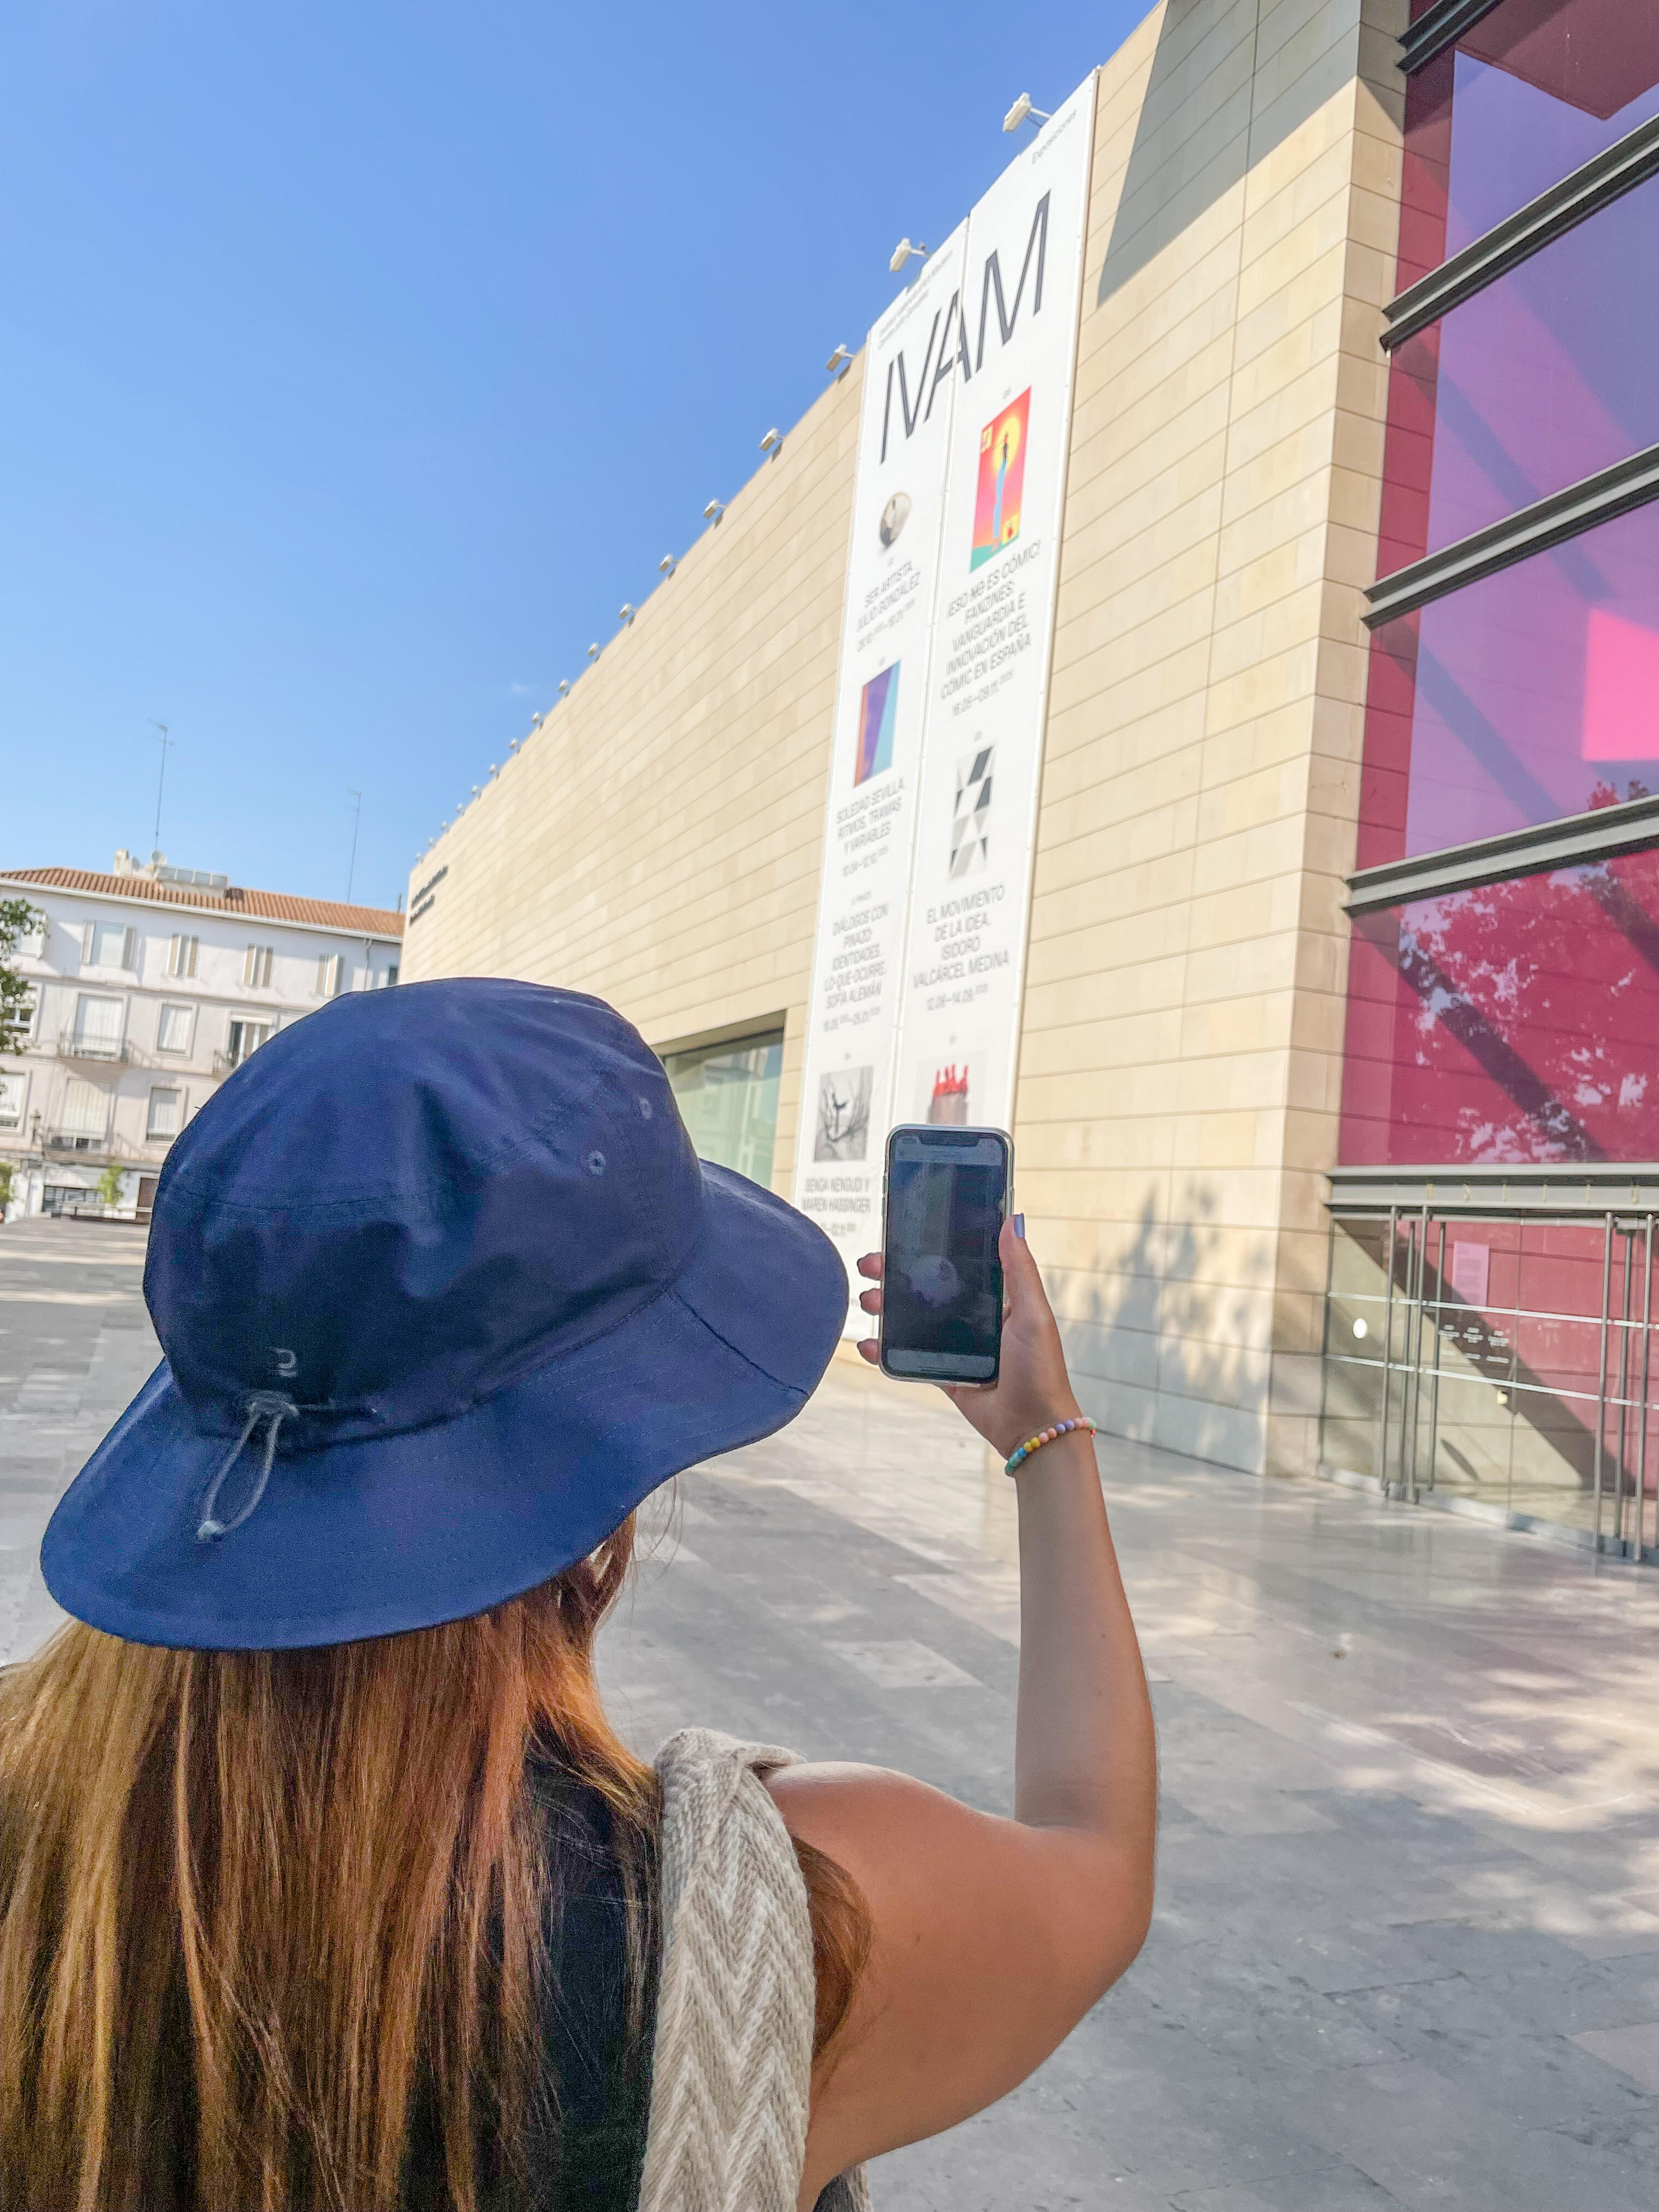
\includegraphics[width=\textwidth]{figs/usuario.jpg}
\end{subfigure}
\hfill
\begin{subfigure}[b]{0.49\textwidth}
    \centering
    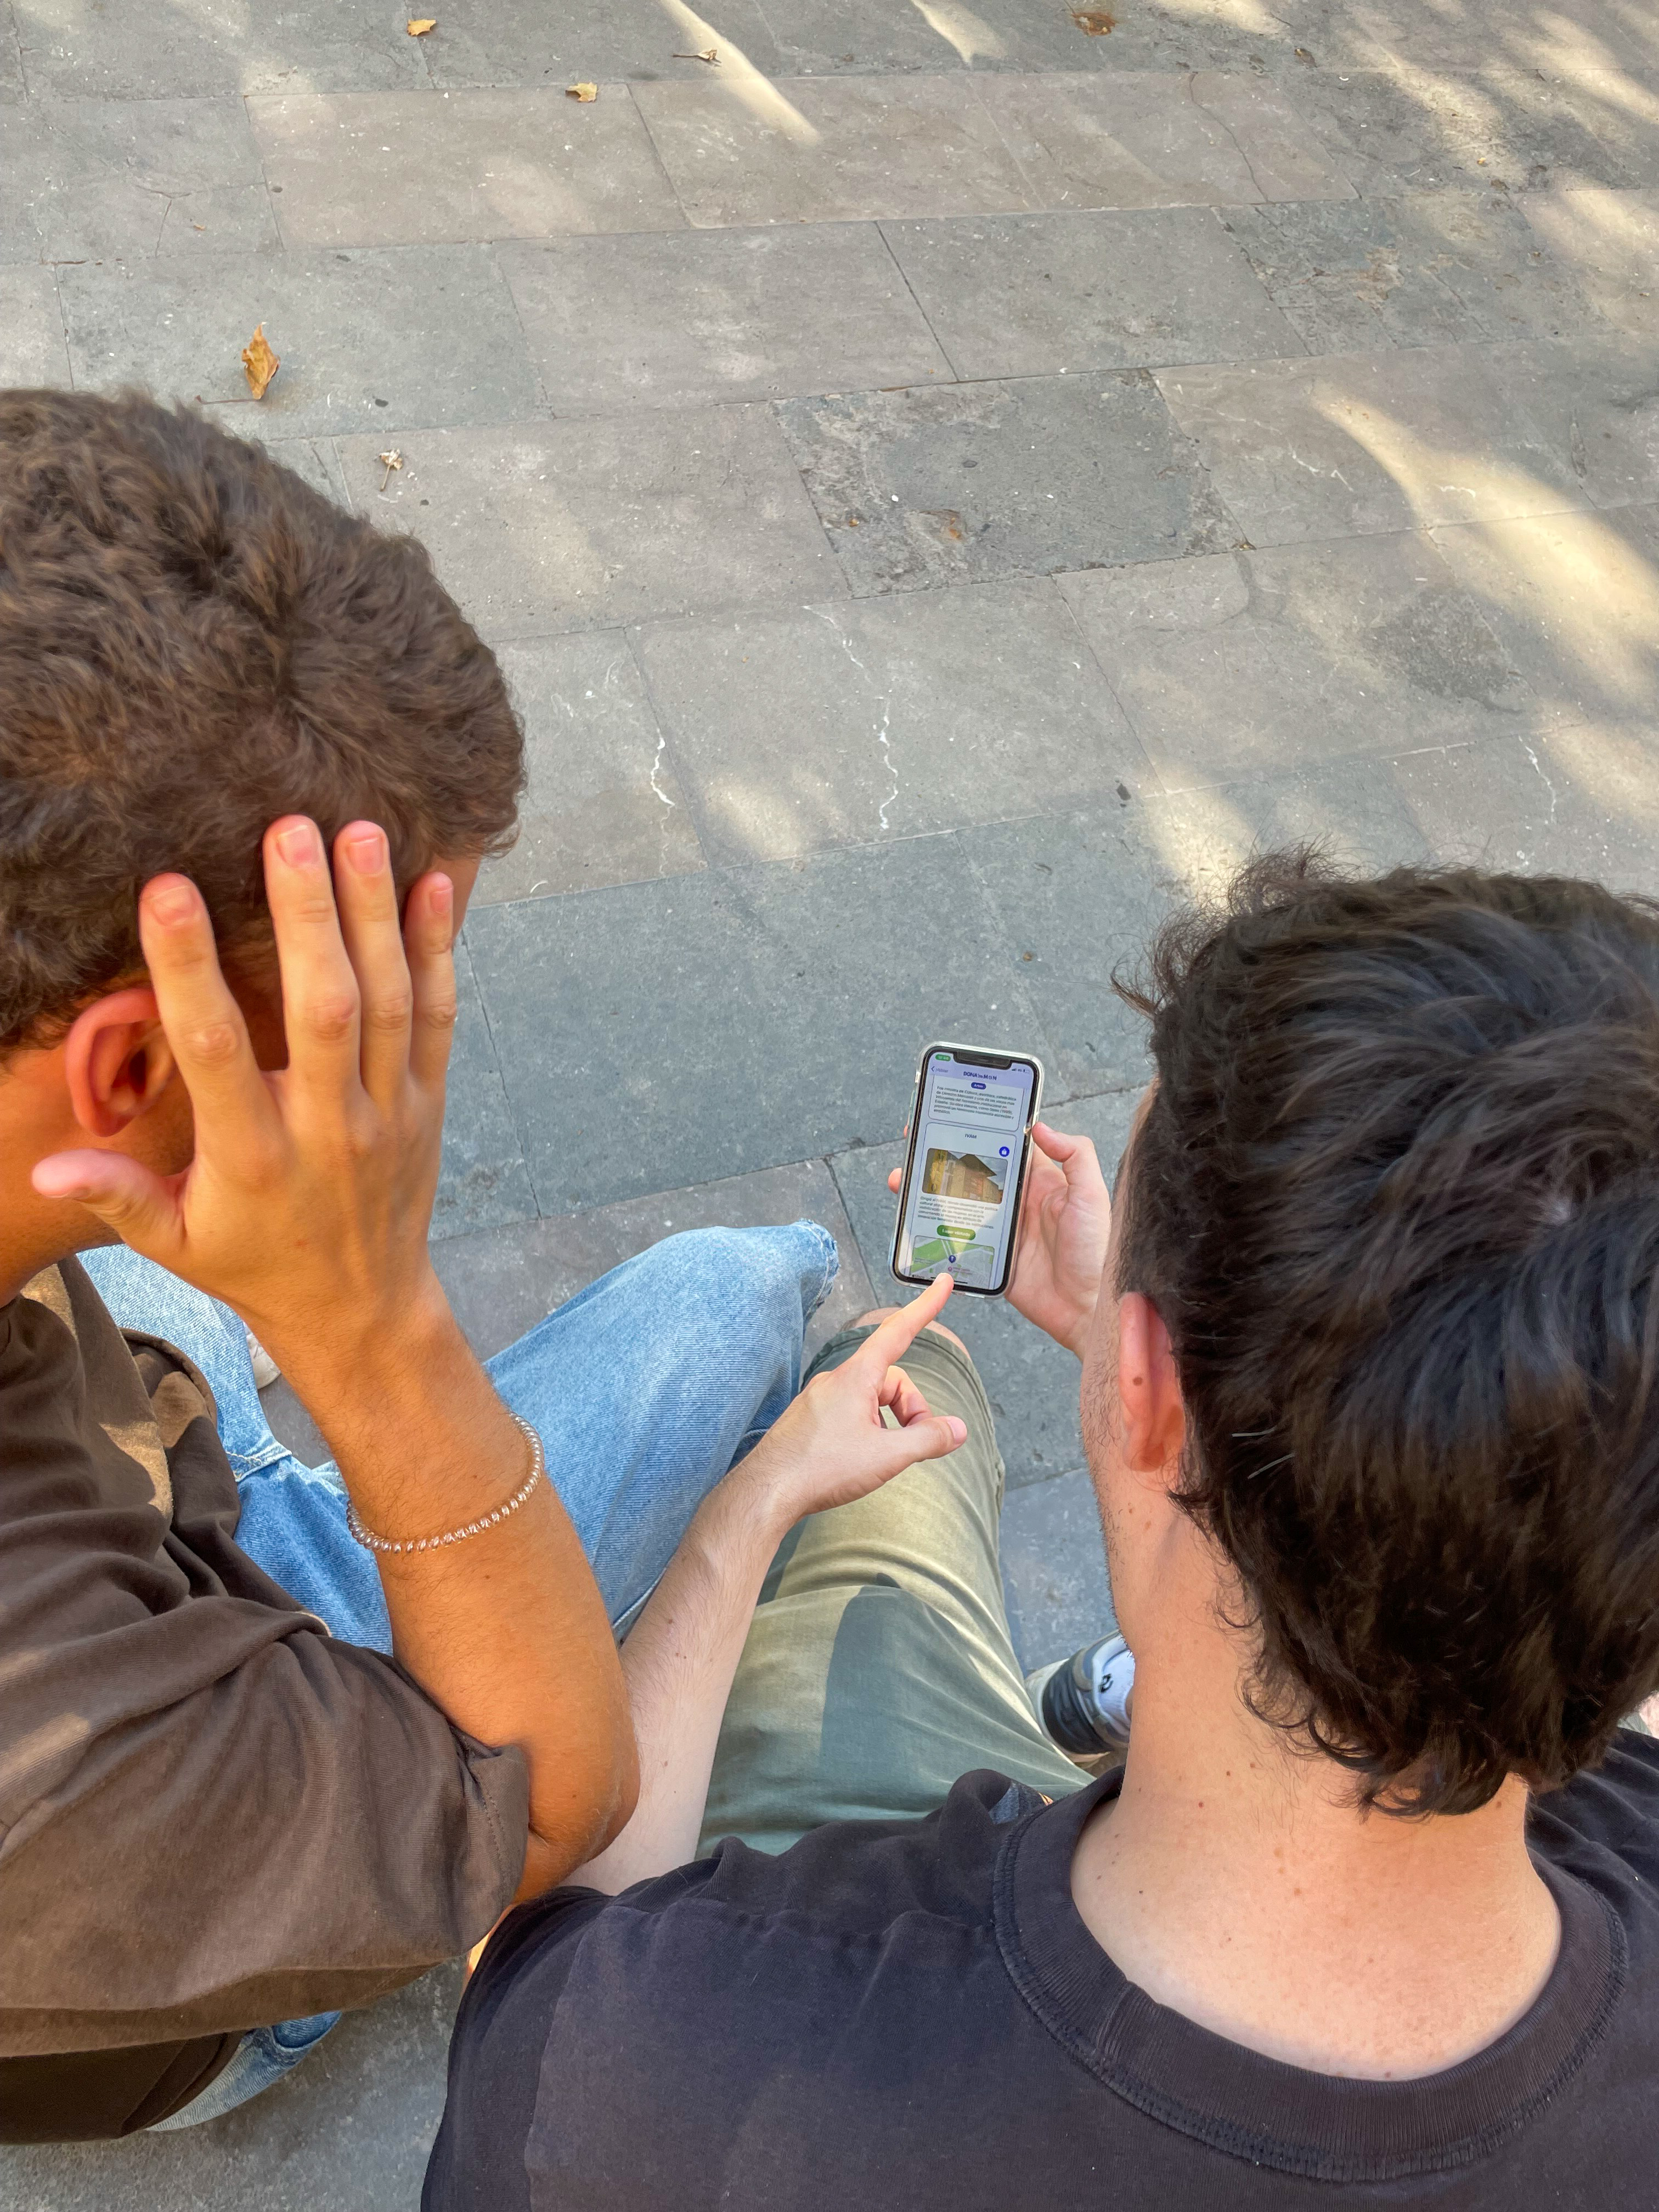
\includegraphics[width=\textwidth]{figs/usuario3.jpg}
\end{subfigure}
\vspace{0.2cm}
\caption{Usuarios probando la aplicación DONA'm MÓN en el IVAM}
\label{fig:usuarios-sus}
\end{figure}

\subsection{Cálculo del SUS}
El cálculo de la puntuación SUS se realiza del siguiente modo:
\begin{itemize}
    \item Para preguntas impares (1, 3, 5, 7, 9): $(\text{valor}) - 1$.
    \item Para preguntas pares (2, 4, 6, 8, 10): $5 - (\text{valor})$.
    \item Se suman los resultados anteriores y se multiplica por 2,5.
\end{itemize}

Ejemplo para U1:
\[
\text{Ajuste} = ((4-1)+(5-1)+(5-1)+(4-1)+(4-1)) + 
\]
\[
((5-1)+(5-2)+(5-1)+(5-1)+(5-1))
\]
\[
\text{Suma total} = 34, \; \text{SUS} = 34 \times 2,5 = 85
\]


\subsection{Resultados del cuestionario}
En la Tabla~\ref{tab:sus-respuestas} se muestran las puntuaciones otorgadas por cada usuario.

\begin{table}[H]
\centering
\renewcommand{\arraystretch}{0.9} % Menos espacio entre filas
\resizebox{0.8\textwidth}{!}{ % Ajusta al 80% del ancho del texto
\begin{tabular}{|c|cccccccccc|}
\hline
\textbf{Usuario} & \textbf{P1} & \textbf{P2} & \textbf{P3} & \textbf{P4} & \textbf{P5} & \textbf{P6} & \textbf{P7} & \textbf{P8} & \textbf{P9} & \textbf{P10} \\
\hline
\multicolumn{11}{|c|}{\textit{Escala: 1 = Totalmente en desacuerdo, 5 = Totalmente de acuerdo}}\\
\hline
U1  & 4 & 1 & 4 & 1 & 5 & 2 & 5 & 1 & 4 & 1 \\
U2  & 4 & 3 & 4 & 2 & 4 & 3 & 4 & 2 & 5 & 2 \\
U3  & 5 & 1 & 5 & 1 & 5 & 1 & 5 & 1 & 5 & 1 \\
U4  & 4 & 1 & 5 & 1 & 5 & 1 & 4 & 1 & 5 & 1 \\
U5  & 4 & 1 & 5 & 1 & 5 & 1 & 5 & 1 & 5 & 5 \\
U6  & 5 & 2 & 4 & 2 & 5 & 1 & 4 & 2 & 5 & 2 \\
U7  & 5 & 2 & 5 & 4 & 4 & 2 & 5 & 2 & 5 & 2 \\
U8  & 4 & 1 & 4 & 4 & 5 & 1 & 4 & 3 & 5 & 2 \\
U9  & 4 & 1 & 5 & 1 & 5 & 2 & 4 & 1 & 5 & 1 \\
U10 & 4 & 1 & 5 & 1 & 4 & 2 & 5 & 1 & 5 & 1 \\
U11 & 5 & 2 & 5 & 1 & 5 & 2 & 5 & 2 & 5 & 2 \\
U12 & 4 & 2 & 5 & 2 & 5 & 2 & 4 & 2 & 4 & 2 \\
U13 & 5 & 1 & 4 & 1 & 5 & 1 & 5 & 2 & 5 & 1 \\
U14 & 4 & 3 & 4 & 2 & 5 & 2 & 4 & 2 & 4 & 2 \\
U15 & 5 & 4 & 5 & 2 & 5 & 1 & 5 & 1 & 5 & 1 \\
U16 & 4 & 1 & 5 & 1 & 4 & 2 & 5 & 2 & 5 & 1 \\
U17 & 5 & 1 & 5 & 2 & 5 & 1 & 5 & 1 & 5 & 1 \\
\hline
\end{tabular}
} % Fin resizebox
\caption{Respuestas del cuestionario SUS por usuario}
\label{tab:sus-respuestas}
\end{table}

\subsection{Visualización de resultados por pregunta}
Además de la tabla general, se presentan a continuación las preguntas del cuestionario SUS junto con las gráficas que ilustran la distribución de respuestas para cada una. Estas visualizaciones permiten comprender de manera más clara la percepción de los usuarios en relación con los distintos aspectos de la usabilidad evaluados.

\textbf{Pregunta 1:} Considero que me gustaría utilizar frecuentemente esta aplicación.

\begin{figure}[H]
\centering
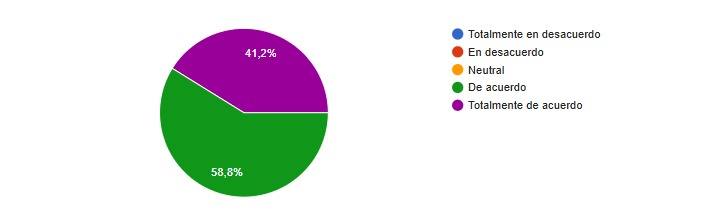
\includegraphics[width=0.7\textwidth]{figs/sus_p1.jpg}
\caption{Distribución de respuestas a la Pregunta 1}
\end{figure}

\textbf{Pregunta 2:} He encontrado la aplicación innecesariamente compleja en algunos momentos.

\begin{figure}[H]
\centering
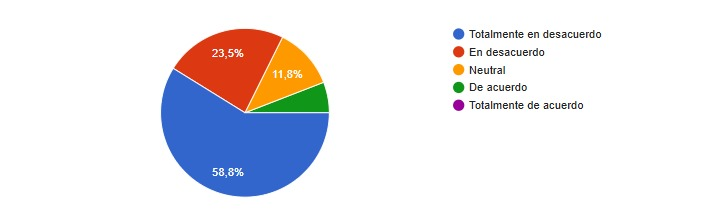
\includegraphics[width=0.7\textwidth]{figs/sus_p2.jpg}
\caption{Distribución de respuestas a la Pregunta 2}
\end{figure}

\textbf{Pregunta 3:} Me ha parecido fácil de usar.

\begin{figure}[H]
\centering
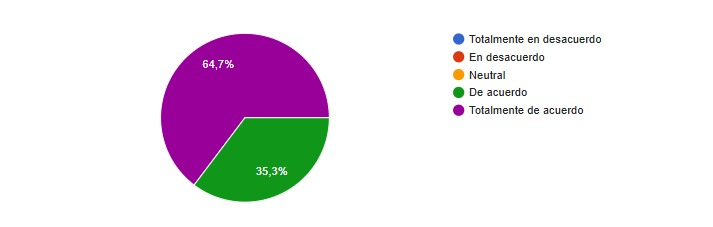
\includegraphics[width=0.7\textwidth]{figs/sus_p3.jpg}
\caption{Distribución de respuestas a la Pregunta 3}
\end{figure}

\textbf{Pregunta 4:} Creo que necesitaría ayuda de una persona con conocimientos técnicos para poder usarla.

\begin{figure}[H]
\centering
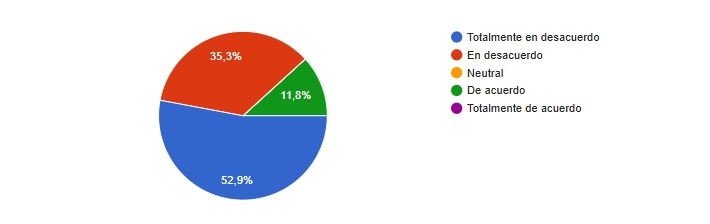
\includegraphics[width=0.7\textwidth]{figs/sus_p4.jpg}
\caption{Distribución de respuestas a la Pregunta 4}
\end{figure}

\textbf{Pregunta 5:} Las funcionalidades están bien integradas y tienen coherencia entre sí.

\begin{figure}[H]
\centering
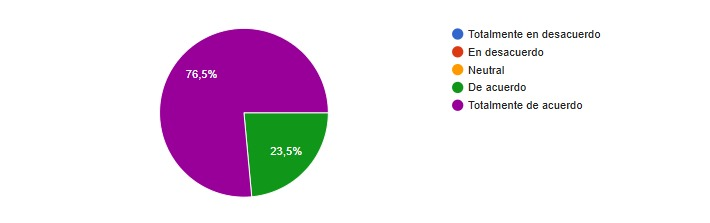
\includegraphics[width=0.7\textwidth]{figs/sus_p5.jpg}
\caption{Distribución de respuestas a la Pregunta 5}
\end{figure}

\textbf{Pregunta 6:} Me parece que hay demasiada inconsistencia en la aplicación.

\begin{figure}[H]
\centering
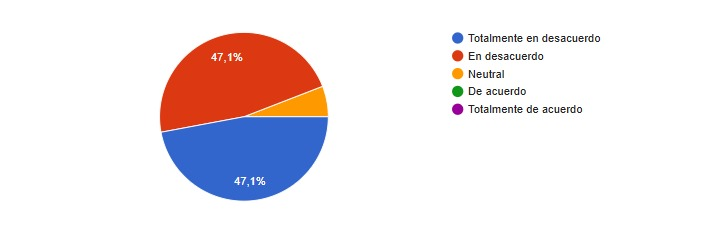
\includegraphics[width=0.7\textwidth]{figs/sus_p6.jpg}
\caption{Distribución de respuestas a la Pregunta 6}
\end{figure}

\textbf{Pregunta 7:} Creo que la mayoría de la gente aprendería a usar esta aplicación con rapidez.

\begin{figure}[H]
\centering
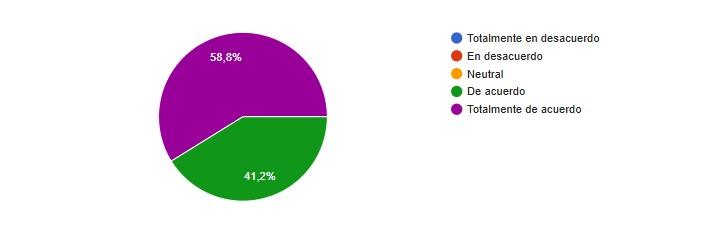
\includegraphics[width=0.7\textwidth]{figs/sus_p7.jpg}
\caption{Distribución de respuestas a la Pregunta 7}
\end{figure}

\textbf{Pregunta 8:} Me ha parecido confusa o difícil de manejar en algunos aspectos.

\begin{figure}[H]
\centering
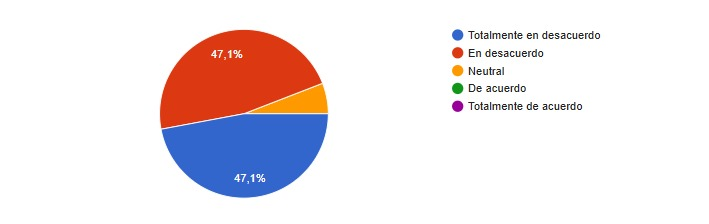
\includegraphics[width=0.7\textwidth]{figs/sus_p8.jpg}
\caption{Distribución de respuestas a la Pregunta 8}
\end{figure}

\textbf{Pregunta 9:} Me he sentido segura usando la aplicación.

\begin{figure}[H]
\centering
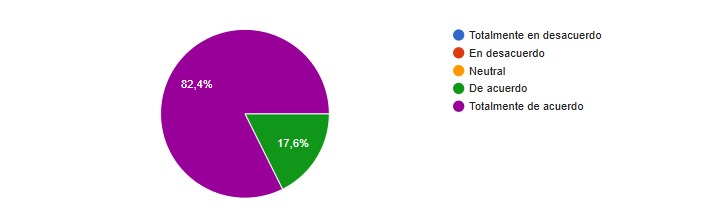
\includegraphics[width=0.7\textwidth]{figs/sus_p9.jpg}
\caption{Distribución de respuestas a la Pregunta 9}
\end{figure}

\textbf{Pregunta 10:} Necesité aprender muchas cosas antes de poder usarla correctamente.

\begin{figure}[H]
\centering
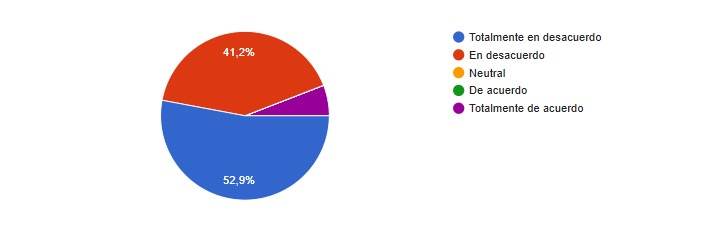
\includegraphics[width=0.7\textwidth]{figs/sus_p10.jpg}
\caption{Distribución de respuestas a la Pregunta 10}
\end{figure}


\subsection{Puntuaciones SUS}
En la Tabla~\ref{tab:sus-final} se muestran las puntuaciones calculadas aplicando la fórmula mencionada anteriormente, junto con información básica sobre los participantes (edad, ocupación y familiaridad con Realidad Aumentada). Cabe destacar que todos los usuarios tienen experiencia utilizando aplicaciones móviles. 

Las edades de los usuarios oscilan principalmente entre los 22 y los 27 años, que es el público objetivo principal de la aplicación. No obstante, también se ha realizado la prueba con usuarios en torno a los 50 años para recoger opiniones y percepciones de otros rangos de edad.
\begin{table}[H]
\centering
\scriptsize
\renewcommand{\arraystretch}{1.2}
\begin{tabular}{|c|c|p{4cm}|c|c|}
\hline
\textbf{Usuario} & \textbf{Edad} & \textbf{Descripción} & \textbf{Familiaridad RA} & \textbf{Puntuación SUS} \\
\hline
U1 & 22 & Estudiante de Bellas Artes & Baja & 85 \\
U2 & 21 & Periodista & Baja & 77,5 \\
U3 & 19 & Estudiante de Óptica y Optometría& Baja & 100 \\
U4 & 24 & Ingeniero en Telecomunicaciones & Media & 95 \\
U5 & 22 & Especialista en marketing & Baja & 92,5 \\
U6 & 22 & Fisioterapeuta & Baja & 90 \\
U7 & 55 & Limpiadora & Baja & 80 \\
U8 & 50 & Instalador del gas & Baja & 82,5 \\
U9 & 24 & Estudiante de Desarrollo Web & Alta & 90 \\
U10 & 22 & Estudiante de Desarrollo Web & Alta & 90 \\
U11 & 24 & Restauradora de Arte & Baja & 87,5 \\
U12 & 27 & Ingeniero Multimedia & Alta & 82,5 \\
U13 & 23 & Ingeniera en Telecomunicaciones & Media & 95 \\
U14 & 23 & Estudiante de Ingeniería Multimedia & Alta & 77,5 \\
U15 & 23 & Dietista & Baja & 87,5 \\
U16 & 24 & Estudiante de Desarrollo Web & Alta & 90 \\
U17 & 22 & Estudiante de Desarrollo Web & Alta & 95 \\
\hline
\textbf{Media} & -- & -- & -- & \textbf{87,65} \\
\hline
\end{tabular}
\caption{Perfil de los participantes y puntuación SUS final}
\label{tab:sus-final}
\end{table}

Los resultados obtenidos reflejan una puntuación media de \textbf{87,65} en la escala SUS, lo que sitúa la aplicación en la categoría \textit{Excelente}. Como se observa en la Figura~\ref{fig:sus-usuarios}, la mayoría de usuarios obtiene puntuaciones superiores a 80, con varios casos alcanzando valores cercanos o iguales a 100. 

La distribución de las puntuaciones SUS por rangos puede verse en la Figura~\ref{fig:sus-distribucion}, donde se aprecia que la mayor parte de los participantes se concentra en los intervalos de 90-99, lo que refuerza la excelente percepción de usabilidad de la aplicación.

\begin{figure}[H]
\centering
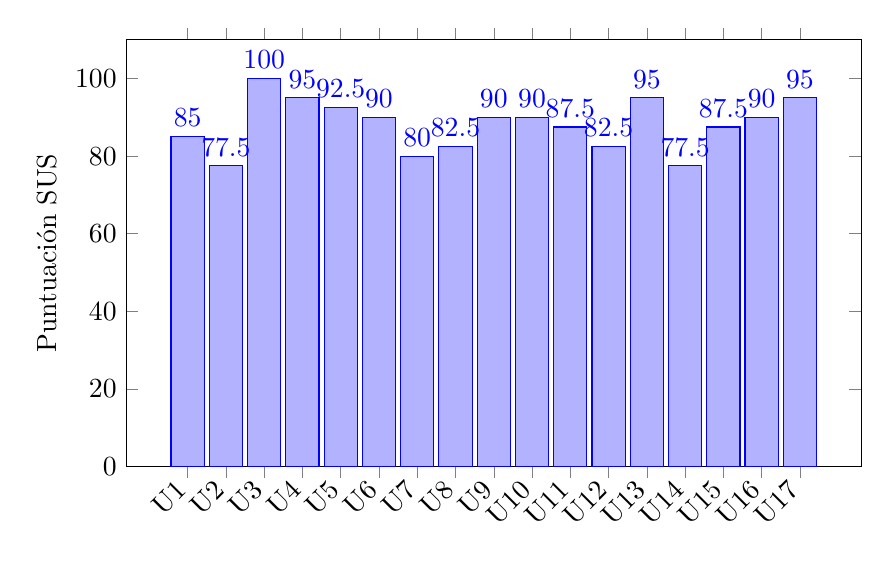
\begin{tikzpicture}
\begin{axis}[
    ybar,
    width=0.9\textwidth,
    height=7cm,
    bar width=12pt,
    ymin=0,
    ymax=110,
    ylabel={Puntuación SUS},
    symbolic x coords={U1,U2,U3,U4,U5,U6,U7,U8,U9,U10,U11,U12,U13,U14,U15,U16,U17},
    xtick=data,
    x tick label style={rotate=45, anchor=east},
    nodes near coords,
    nodes near coords align={vertical},
]
\addplot coordinates {(U1,85)(U2,77.5)(U3,100)(U4,95)(U5,92.5)(U6,90)(U7,80)(U8,82.5)(U9,90)(U10,90)(U11,87.5)(U12,82.5)(U13,95)(U14,77.5)(U15,87.5)(U16,90)(U17,95)};
\end{axis}
\end{tikzpicture}
\caption{Puntuaciones SUS por usuario.}
\label{fig:sus-usuarios}
\end{figure}

\begin{figure}[H]
\centering
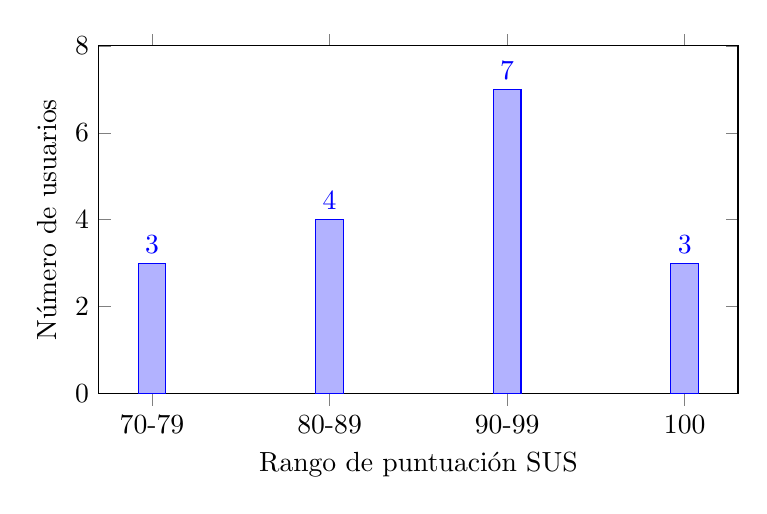
\begin{tikzpicture}
\begin{axis}[
    ybar,
    width=0.8\textwidth,
    height=6cm,
    ymin=0,
    ymax=8,
    ylabel={Número de usuarios},
    xlabel={Rango de puntuación SUS},
    symbolic x coords={70-79,80-89,90-99,100},
    xtick=data,
    nodes near coords,
    nodes near coords align={vertical},
]
\addplot coordinates {(70-79,3)(80-89,4)(90-99,7)(100,3)};
\end{axis}
\end{tikzpicture}
\caption{Distribución de puntuaciones SUS.}
\label{fig:sus-distribucion}
\end{figure}

\subsection{Comentarios adicionales de los usuarios}
Además del cuestionario SUS, se realizaron preguntas abiertas para obtener una visión más cualitativa de la experiencia. A continuación, se destacan las más relevantes:

\textbf{¿Qué parte de la aplicación te ha resultado más útil o interesante?}
\begin{itemize}
    \item \textit{“Las rutas de mujeres destacadas”}.
    \item \textit{“La parte de la realidad aumentada”}.
    \item \textit{“El mapa interactivo, es muy innovador y curioso”}.
    \item \textit{“Como aspecto más interesante e innovador destacaría la opción para hacer rutas en base a las distintas ubicaciones. También es interesante poder ver la fecha en la que visitaste cada lugar”}.
    \item \textit{“Cuando sale en 3D la mujer”}.
\end{itemize}

\textbf{¿Has encontrado algún problema mientras usabas la app?}
\begin{itemize}
    \item La mayoría respondió \textit{“No”} o \textit{“Ninguno en general, el funcionamiento es completamente satisfactorio”}.
    \item Solo un usuario opino que: \textit{“La Realidad Aumentada es un poco difícil de usar”}.
\end{itemize}

\textbf{¿Te ha parecido intuitiva la navegación entre pantallas?}
\begin{itemize}
    \item Comentarios más repetidos: \textit{“Sí, es muy fácil de usar, además está todo muy bien relacionado”}, \textit{“Muy sencilla e intuitiva”}.
\end{itemize}

\textbf{¿Has disfrutado la experiencia de realidad aumentada? ¿Por qué?}
\begin{itemize}
    \item \textit{“Es mi parte favorita de la app, es muy entretenida y original”}.
    \item \textit{“Es fascinante, hace que la app sea mucho más inmersiva”}.
    \item \textit{“Aporta un elemento diferente en comparación con otras aplicaciones”}.
    \item Solo una respuesta negativa: \textit{“No mucho, nunca me ha gustado la RA en aplicaciones”}.
\end{itemize}

\textbf{¿Consideras que la aplicación te ha permitido descubrir información nueva o interesante sobre las mujeres de Valencia?}
\begin{itemize}
    \item \textit{“Sí, es necesario tener herramientas que nos permitan conocer más sobre las acciones que las mujeres han hecho durante la historia”}.
    \item \textit{“Por supuesto, además de añadir conocimientos de valor acerca de nuestra cultura”}.
\end{itemize}

\textbf{¿Recomendarías esta aplicación a otras personas?}
\begin{itemize}
    \item Todas las respuestas fueron afirmativas: \textit{“Por supuesto!!!!”}, \textit{“Si están interesadas en aprender sobre el tema, sin duda”}.
\end{itemize}

\textbf{¿Alguna sugerencia para mejorar la aplicación?}
\begin{itemize}
    \item La mayoría respondió \textit{“No”} o \textit{“Está todo correcto”}.
    \item Comentarios destacados: \textit{“Tal vez un enlace para ampliar aún más la información de cada protagonista”}, \textit{“Que los usuarios puedan recomendar nuevos puntos de interés”}.
\end{itemize}

Podemos concluir, basándonos en los comentarios de los usuarios, que han percibido la navegación como intuitiva y sencilla. Han destacando la coherencia entre las distintas secciones y la facilidad para acceder a la información. Las funcionalidades principales, en particular el mapa interactivo, las rutas temáticas y la experiencia de Realidad Aumentada, se consolidan como los aspectos más valorados, ya que aportan dinamismo y un carácter innovador frente a otras aplicaciones similares. Además, se han propuesto mejoras que se han añadido a la lista de trabajo a futuro.

\section{Hardware empleado en las Pruebas de rendimiento}

Las pruebas de rendimiento se llevaron a cabo en un único equipo portátil para el backend y en un dispositivo móvil para el frontend y la experiencia de realidad aumentada. En la tabla \ref{tab:hardware} se detallan las características técnicas de ambos dispositivos, ya que estas especificaciones pueden influir en los resultados obtenidos.
\begin{table}[H]
\centering
\caption{Especificaciones del hardware utilizado en las pruebas}
\label{tab:hardware}
\renewcommand{\arraystretch}{1.1}
\begin{tabular}{|p{3.2cm}|p{5.7cm}|p{5.2cm}|}
\hline
\textbf{Componente} & \textbf{Portátil \cite{asus_rog_strix}} & \textbf{Móvil \cite{iphone_11_specs}} \\
\hline
Modelo & Asus ROG Strix G15 G513IC-HN004 & iPhone 11 \\
\hline
Procesador & AMD Ryzen 7 4800H (8 núcleos, 2.9-4.2 GHz) & A13 Bionic (6 núcleos) \\
\hline
Memoria RAM & 16 GB DDR4 a 3200 MHz & 4 GB \\
\hline
Almacenamiento & 512 GB SSD M.2 NVMe PCIe & 64 GB \\
\hline
GPU & NVIDIA GeForce RTX 3050, 4 GB GDDR6 & GPU Apple de 4 núcleos \\
\hline
Pantalla & 15.6" Full HD, 144 Hz & 6.1" Liquid Retina HD (1792 x 828) \\
\hline
Sistema operativo & Windows 11 Home & iOS 18.5 \\
\hline
Conectividad & Wi-Fi 6, Bluetooth 5.1 & Wi-Fi 802.11ax, Bluetooth 5.0 \\
\hline
\end{tabular}
\end{table}



\section{Pruebas de Rendimiento del Backend}

\subsection{Metodología}

Para comprobar el rendimiento del backend, se han realizado pruebas con \textbf{Apache JMeter} \cite{apache_jmeter}, simulando condiciones de uso normal y situaciones extremas. Se han analizado métricas como el tiempo de respuesta (desde que se envía la petición hasta que llega la respuesta), percentiles para entender la distribución, la desviación estándar para medir estabilidad, el throughput (peticiones procesadas por segundo) y el porcentaje de errores.

\subsubsection{Configuración de Pruebas}

Se definieron dos escenarios:

\begin{itemize}
    \item \textbf{Carga Normal}: 10 usuarios concurrentes, 10 iteraciones por usuario (100 peticiones por endpoint) y usuarios añadidos progresivamente durante 5 segundos (ramp-up de 5 s).
    \item \textbf{Carga de Estrés}: 50 usuarios concurrentes, 20 iteraciones por usuario (1000 peticiones por endpoint) y usuarios añadidos progresivamente durante 10 segundos (ramp-up de 10 s).
\end{itemize}

Los endpoints evaluados corresponden a las principales operaciones: autenticación (\textit{Login}), lectura de datos (\textit{GET Mujeres}, \textit{GET Lugares}, \textit{GET Rutas}, \textit{GET Visited Lugares}) y escritura (\textit{POST Visit Lugar}, \textit{POST Visit Lugar Ruta}). Todos, salvo \textit{Login}, requieren autenticación JWT.

\subsection{Resultados y Análisis}

\subsubsection{Carga Normal}

La Tabla \ref{tab:normal} muestra los resultados con 10 usuarios concurrentes. Se incluyen el tiempo medio (\textbf{Avg}), valores percentiles (P90, P95), máximo, desviación estándar y throughput.

\begin{table}[H]
\centering
\caption{Resultados bajo carga normal (10 usuarios, 100 peticiones por endpoint)}
\label{tab:normal}
\scriptsize
\begin{tabular}{|l|c|c|c|c|c|c|c|c|c|}
\hline
\textbf{Endpoint} & \textbf{Avg} & \textbf{Min} & \textbf{Median} & \textbf{P90} & \textbf{P95} & \textbf{Max} & \textbf{Std Dev} & \textbf{Throughput} & \textbf{Error\%} \\
\hline
Login & 458 & 358 & 460 & 500 & 519 & 529 & 36.0 & 8.22 & 0 \\
GET Mujeres & 37 & 20 & 34 & 54 & 66 & 80 & 13.7 & 8.46 & 0 \\
GET Lugares & 42 & 20 & 38 & 65 & 72 & 126 & 19.1 & 8.46 & 0 \\
GET Rutas & 54 & 27 & 48 & 81 & 100 & 153 & 22.8 & 8.44 & 0 \\
POST Visit Lugar & 67 & 53 & 64 & 79 & 86 & 99 & 9.9 & 8.42 & 0 \\
POST Visit Lugar Ruta & 70 & 59 & 69 & 88 & 89 & 119 & 11.1 & 8.42 & 0 \\
GET Visited Lugares & 71 & 58 & 69 & 89 & 89 & 120 & 11.9 & 8.42 & 0 \\
\hline
\end{tabular}
\end{table}
Bajo carga normal, el sistema presenta un comportamiento óptimo tanto en velocidad como en estabilidad. Como se aprecia en la Tabla \ref{tab:normal}, la mayoría de endpoints procesan las peticiones en menos de 100 ms, garantizando una experiencia de usuario fluida y sin retardos perceptibles.

Las operaciones de lectura destacan por su rapidez: \textit{GET Mujeres} responde en apenas 37 ms, y \textit{GET Lugares} en 42 ms, valores excelentes considerando que implican consultas y serialización de datos JSON. Incluso \textit{GET Rutas}, con 54 ms, mantiene tiempos muy bajos. Las operaciones de escritura (\textit{POST Visit Lugar} y \textit{POST Visit Lugar Ruta}) son ligeramente más costosas, situándose en torno a 67-70 ms, debido a la validación de datos y la inserción en base de datos, pero siguen siendo muy rápidas.

El único endpoint que supera los 400 ms es \textit{Login} (458 ms), lo cual era esperado porque incluye la generación y firma criptográfica del token JWT, una operación CPU-bound.

La baja desviación estándar ($\leq$ 36 ms en todos los casos) evidencia que la latencia es estable y predecible, sin picos relevantes. Además, no se registraron errores (0) y el throughput ronda las 8.4 req/s, lo que indica que el backend no solo es rápido, sino también consistente. 
\subsubsection{Carga de Estrés}

La Tabla \ref{tab:stress} presenta los resultados con 50 usuarios y 1000 peticiones por endpoint.

\begin{table}[H]
\centering
\caption{Resultados bajo carga de estrés (50 usuarios, 1000 peticiones por endpoint)}
\label{tab:stress}
\scriptsize
\begin{tabular}{|l|c|c|c|c|c|c|c|c|c|}
\hline
\textbf{Endpoint} & \textbf{Avg} & \textbf{Min} & \textbf{Median} & \textbf{P90} & \textbf{P95} & \textbf{Max} & \textbf{Std Dev} & \textbf{Throughput} & \textbf{Error\%} \\
\hline
Login & 1154 & 371 & 1150 & 1490 & 1659 & 2155 & 279.6 & 8.81 & 0 \\
GET Mujeres & 674 & 24 & 696 & 902 & 968 & 1429 & 207.6 & 8.82 & 0 \\
GET Lugares & 783 & 23 & 806 & 1014 & 1096 & 1779 & 226.8 & 8.78 & 0 \\
GET Rutas & 892 & 26 & 901 & 1147 & 1227 & 1788 & 225.5 & 8.75 & 0 \\
POST Visit Lugar & 613 & 60 & 634 & 794 & 841 & 1477 & 176.3 & 8.75 & 0 \\
POST Visit Lugar Ruta & 571 & 60 & 590 & 760 & 810 & 1419 & 183.3 & 8.75 & 0 \\
GET Visited Lugares & 554 & 69 & 570 & 741 & 809 & 1084 & 177.1 & 8.74 & 0 \\
\hline
\end{tabular}
\end{table}
Bajo carga de estrés, la latencia aumenta significativamente, especialmente en operaciones de lectura (\textit{GET}), que llegan a 892 ms en \textit{GET Rutas} y 783 ms en \textit{GET Lugares}. Las operaciones de escritura escalan mejor, aunque también se incrementan a valores cercanos a 600 ms. El endpoint \textit{Login} alcanza 1154 ms, pero mantiene una degradación proporcionalmente menor ($\approx$2.5x).

A pesar del aumento, la ausencia de errores y un throughput constante de 8.7 req/s demuestran que el sistema sigue siendo estable y no pierde peticiones, sacrificando únicamente velocidad. Sin embargo, estos tiempos podrían impactar la experiencia en escenarios de alta concurrencia prolongada, lo que sugiere que optimizaciones a nivel de consultas y cacheado serían recomendables para mejorar la escalabilidad.

\textbf{Interpretación AVG:} La Figura \ref{fig:avg_compare} muestra cómo los tiempos promedio bajo estrés aumentan significativamente en comparación con la carga normal. Operaciones de lectura (\textit{GET}) son las más afectadas, alcanzando entre 674 ms y 892 ms, mientras que las de escritura (\textit{POST}) escalan mejor.




\begin{figure}[H]
\centering
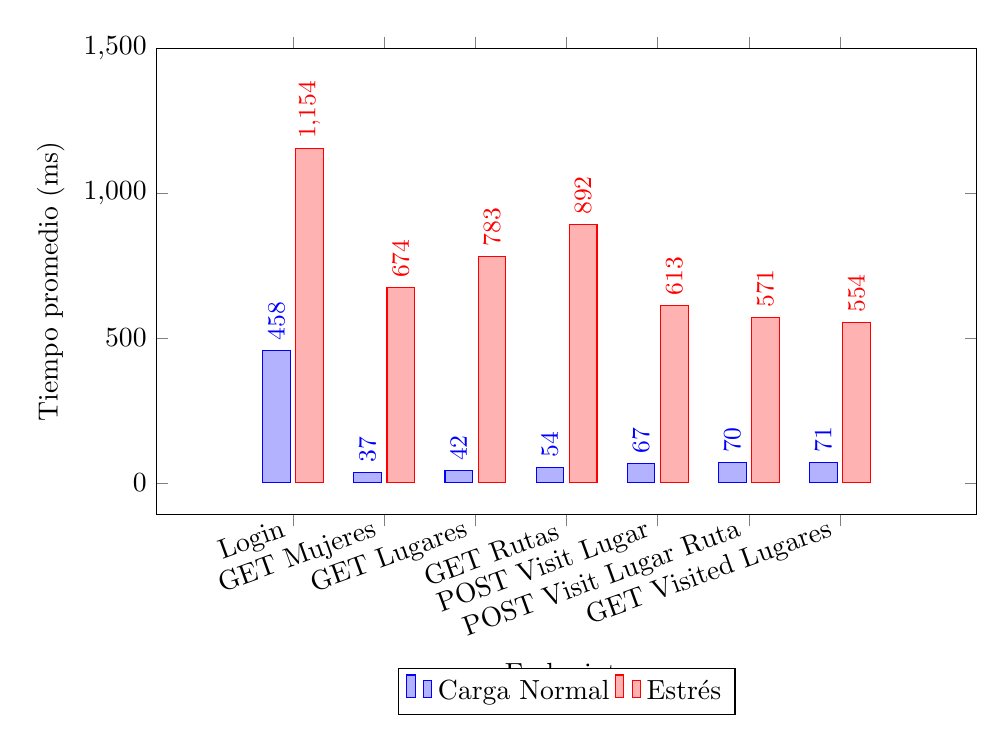
\begin{tikzpicture}
\begin{axis}[
    width=12cm, height=7.5cm,
    ybar,
    bar width=10pt,
    enlarge x limits=0.25,
    ylabel={Tiempo promedio (ms)},
    xlabel={Endpoints},
    symbolic x coords={Login, GET Mujeres, GET Lugares, GET Rutas, POST Visit Lugar, POST Visit Lugar Ruta, GET Visited Lugares},
    xtick=data,
    x tick label style={rotate=20, anchor=east},
    legend style={at={(0.5,-0.33)},anchor=north,legend columns=-1},
    nodes near coords,
    every node near coord/.append style={font=\small, rotate=90, anchor=west},
    ymax=1500,
]
\addplot coordinates {(Login,458) (GET Mujeres,37) (GET Lugares,42) (GET Rutas,54) (POST Visit Lugar,67) (POST Visit Lugar Ruta,70) (GET Visited Lugares,71)};
\addplot coordinates {(Login,1154) (GET Mujeres,674) (GET Lugares,783) (GET Rutas,892) (POST Visit Lugar,613) (POST Visit Lugar Ruta,571) (GET Visited Lugares,554)};
\legend{Carga Normal, Estrés}
\end{axis}
\end{tikzpicture}
\caption{Comparación de tiempos promedio por endpoint}
\label{fig:avg_compare}
\end{figure}


\textbf{Interpretación P95:} El percentil 95 refleja el tiempo que tarda el 95\% de las peticiones en completarse. Como se ve en la Figura \ref{fig:p95_compare}, bajo carga normal la mayoría de endpoints se mantienen por debajo de 100 ms, excepto \textit{Login}. Bajo estrés, el P95 alcanza 1659 ms en \textit{Login} y 1227 ms en \textit{GET Rutas}, lo que indica que las colas de espera y la saturación afectan significativamente la experiencia.

\begin{figure}[H]
\centering
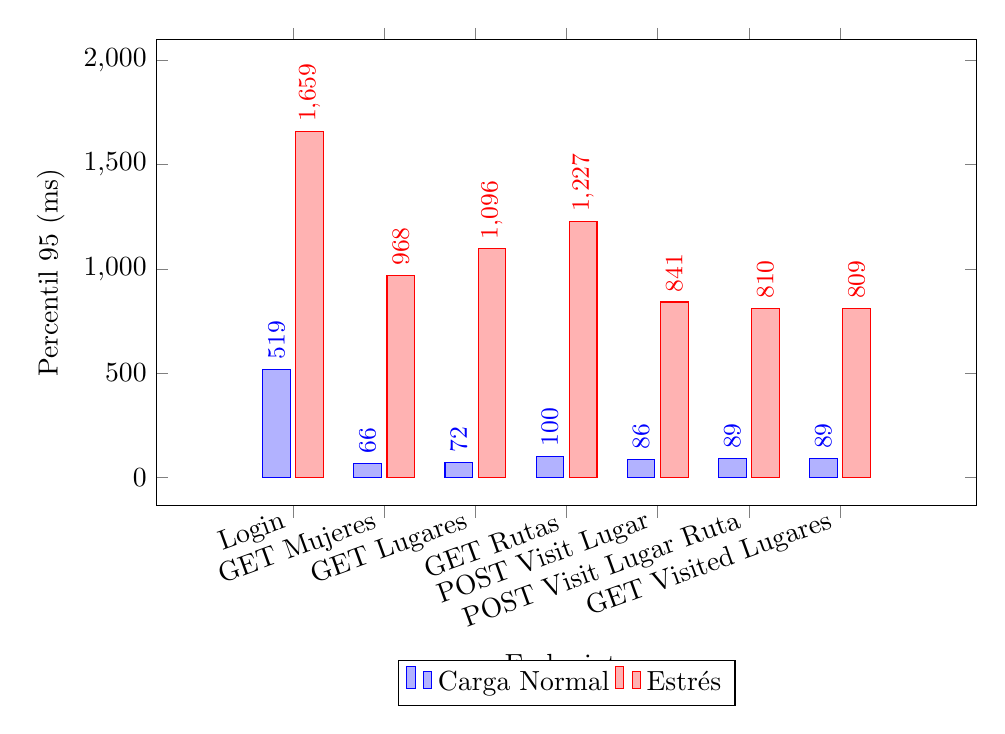
\begin{tikzpicture}
\begin{axis}[
    width=12cm, height=7.5cm,
    ybar,
    bar width=10pt,
    enlarge x limits=0.25,
    ylabel={Percentil 95 (ms)},
    xlabel={Endpoints},
    symbolic x coords={Login, GET Mujeres, GET Lugares, GET Rutas, POST Visit Lugar, POST Visit Lugar Ruta, GET Visited Lugares},
    xtick=data,
    x tick label style={rotate=20, anchor=east},
    legend style={at={(0.5,-0.33)},anchor=north,legend columns=-1},
    nodes near coords,
    every node near coord/.append style={font=\small, rotate=90, anchor=west},
    ymax=2100,
]
\addplot coordinates {(Login,519) (GET Mujeres,66) (GET Lugares,72) (GET Rutas,100) (POST Visit Lugar,86) (POST Visit Lugar Ruta,89) (GET Visited Lugares,89)};
\addplot coordinates {(Login,1659) (GET Mujeres,968) (GET Lugares,1096) (GET Rutas,1227) (POST Visit Lugar,841) (POST Visit Lugar Ruta,810) (GET Visited Lugares,809)};
\legend{Carga Normal, Estrés}
\end{axis}
\end{tikzpicture}
\caption{Comparación del percentil 95 por endpoint}
\label{fig:p95_compare}
\end{figure}

\textbf{Interpretación Max:} El tiempo máximo representa los casos más extremos. En la Figura \ref{fig:max_compare} se aprecia que bajo estrés los picos superan los 2 segundos en \textit{Login} y alcanzan casi 1.8 segundos en operaciones de lectura. Aunque son valores excepcionales, son importantes porque pueden impactar la percepción de fluidez.

\begin{figure}[H]
\centering
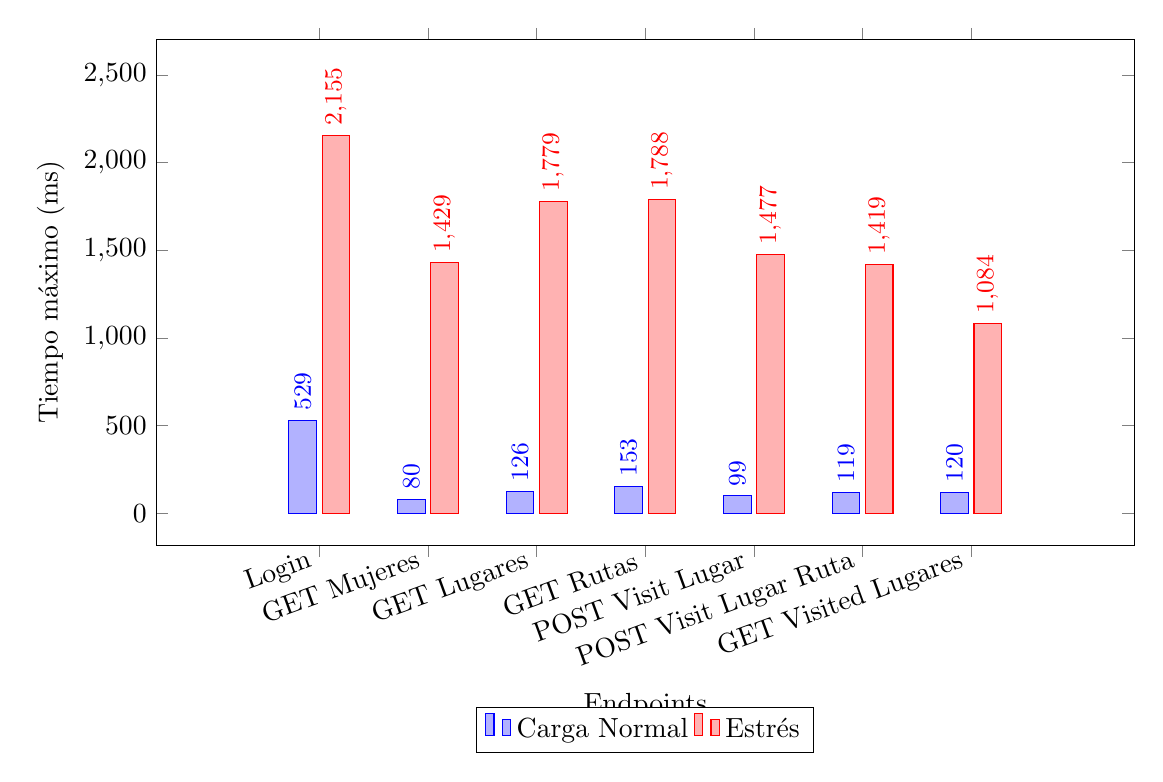
\begin{tikzpicture}
\begin{axis}[
    width=14cm, height=8cm,
    ybar,
    bar width=10pt,
    enlarge x limits=0.25,
    ylabel={Tiempo máximo (ms)},
    xlabel={Endpoints},
    symbolic x coords={Login, GET Mujeres, GET Lugares, GET Rutas, POST Visit Lugar, POST Visit Lugar Ruta, GET Visited Lugares},
    xtick=data,
    x tick label style={rotate=20, anchor=east},
    legend style={at={(0.5,-0.32)},anchor=north,legend columns=-1}, % <-- valor más negativo para bajar la leyenda
    nodes near coords,
    every node near coord/.append style={font=\small, rotate=90, anchor=west},
    ymax=2700,
]
\addplot coordinates {(Login,529) (GET Mujeres,80) (GET Lugares,126) (GET Rutas,153) (POST Visit Lugar,99) (POST Visit Lugar Ruta,119) (GET Visited Lugares,120)};
\addplot coordinates {(Login,2155) (GET Mujeres,1429) (GET Lugares,1779) (GET Rutas,1788) (POST Visit Lugar,1477) (POST Visit Lugar Ruta,1419) (GET Visited Lugares,1084)};
\vspace{0.3cm}
\legend{Carga Normal, Estrés}
\end{axis}
\end{tikzpicture}
\vspace{0.3cm}
\caption{Comparación de tiempos máximos por endpoint}
\label{fig:max_compare}
\end{figure}

\subsection*{Conclusión Global}

El sistema muestra un diseño estable y escalable. Bajo carga normal, los tiempos son óptimos (<100 ms en casi todos los endpoints) y sin errores. Bajo estrés, la degradación es significativa (P95 hasta 1659 ms), pero el throughput se mantiene (8.7 req/s) y la tasa de error sigue en 0\%, lo que confirma que el backend soporta alta concurrencia sin fallos, aunque la latencia pueda afectar la UX en escenarios extremos.

\subsection{Pruebas de Rendimiento del Frontend}

Para evaluar el rendimiento del frontend de la aplicación, se ha utilizado la herramienta \textit{Performance Monitor} integrada en \textbf{Expo Go}. Esta permite monitorizar métricas clave como el uso de memoria, la tasa de fotogramas por segundo (\textit{frames per second, FPS}) y la inicialización de módulos nativos, entre otros.

En la Figura \ref{fig:performance_monitor} se muestra la interfaz de la aplicación junto con el panel de información proporcionado. Entre los parámetros monitorizados destacan:

\begin{itemize}
    \item \textbf{Uso de RAM:} Durante la ejecución normal, el consumo promedio de memoria se situó en torno a \textbf{430 MB}.
    \item \textbf{Velocidad de actualización (FPS):} 
    \begin{itemize}
        \item En el hilo de interfaz de usuario (\textit{UI thread}), los FPS se mantuvieron de forma constante en \textbf{60}, salvo en operaciones más exigentes como aplicar filtros o compartir contenido, donde se observó una caída puntual a \textbf{58 FPS} durante aproximadamente un segundo.
        \item En el hilo de JavaScript (\textit{JS thread}), la frecuencia también se mantuvo estable en \textbf{60 FPS} en condiciones normales, pero se redujo a \textbf{51 FPS} en acciones que requieren procesamiento adicional (por ejemplo, filtrado y compartición). Durante la navegación entre pantallas, el promedio del hilo de JavaScript se situó en torno a \textbf{55 FPS}.
    \end{itemize}
    \item \textbf{Inicialización y carga de scripts:} Los valores relacionados con la descarga y ejecución del \textit{bundle} (e.g., \textit{ScriptDownload}, \textit{ScriptExecution}, \textit{RAMBundleLoad}) se mantuvieron en \textbf{0 ms}, reflejando que la aplicación ya se encontraba completamente cargada en el momento de la prueba.
\end{itemize}

En general, los resultados demuestran que se mantiene una experiencia fluida incluso en operaciones que implican renderizado adicional, con un consumo de memoria dentro de lo esperado.



\begin{figure}[H]
    \centering
    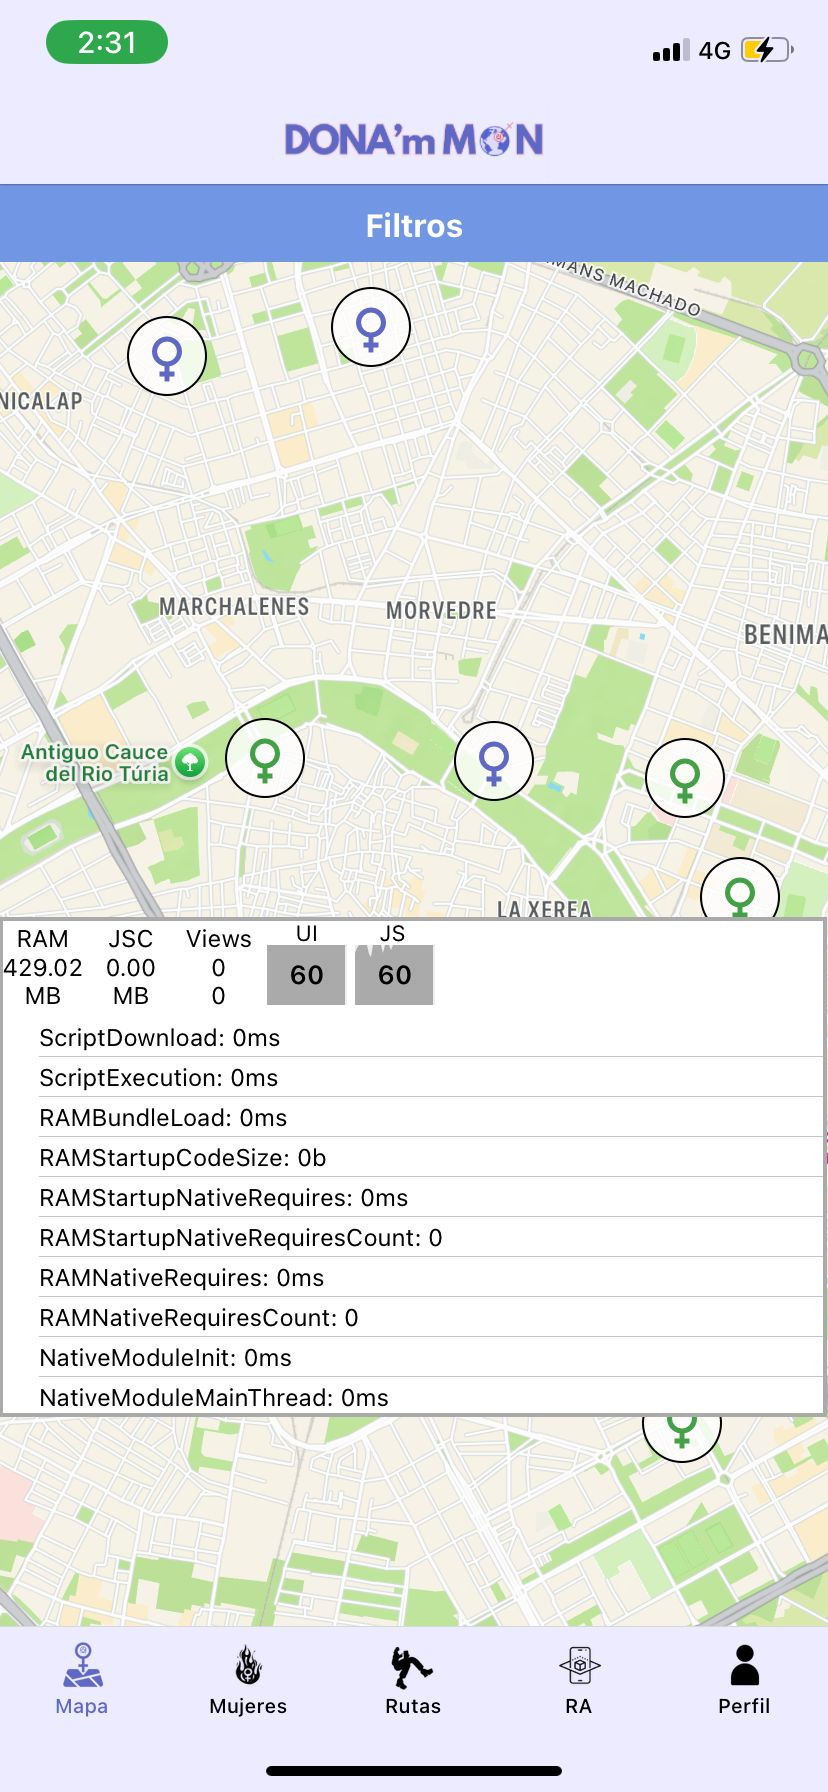
\includegraphics[width=0.5\textwidth]{figs/performance_monitor.jpg}
    \caption{Aplicación DONA'm MÓN ejecutándose en Expo Go con el panel \textit{Performance Monitor}.}
    \label{fig:performance_monitor}
\end{figure}


\section{Pruebas de Rendimiento de la Realidad Aumentada}

Para evaluar el rendimiento de la experiencia de realidad aumentada implementada con A-Frame y AR.js, se han realizado pruebas sobre la versión desplegada en \textit{Vercel} (\url{https://ivam.vercel.app/}) representando el entorno real de uso. El objetivo fue medir el comportamiento en términos de tiempos de carga y estabilidad del renderizado (FPS) durante la interacción del usuario.

\subsection{Metodología}
Se adaptó el código mediante un componente propio en A-Frame que registraba datos de rendimiento en consola, visibles en el dispositivo móvil gracias a la librería \texttt{Eruda}~\cite{eruda}. Estos registros podían consultarse directamente en el dispositivo móvil mediante la consola, como se muestra en la Figura~\ref{fig:captura-logs}. 
\begin{figure}[H]
\centering
\fbox{
\includegraphics[width=0.4\textwidth]{captura_logs.jpg}}
\caption{Captura de los registros obtenidos en el dispositivo durante la prueba}
\label{fig:captura-logs}
\end{figure}

Los parámetros evaluados fueron:
\begin{itemize}
    \item \textbf{Tiempo de carga inicial:} desde la carga de la página hasta la activación de la cámara AR.
    \item \textbf{Carga de modelos 3D:} tiempo exacto en que cada modelo (mundo, lupa, mujer) se encontraba disponible en la escena.
    \item \textbf{Evolución del FPS:} tasa de frames por segundo antes y después de interacciones críticas.
\end{itemize}

Para registrar los valores se añadió el siguiente código JavaScript:

\begin{lstlisting}[language=Python, caption={Fragmento de código para medición de FPS y eventos clave}]
const startTime = performance.now();
AFRAME.registerComponent('fps-logger', {
  tick: function (time, delta) {
    const fps = 1000 / delta;
    if (Math.floor(time) % 1000 === 0) console.log('FPS:', fps.toFixed(2));
  }
});
document.querySelector('#mundoModel').addEventListener('model-loaded', () =>
  console.log('Modelo MUNDO cargado en:', ((performance.now() - startTime)/1000).toFixed(2), 's')
);
document.querySelector('#lupaModel').addEventListener('model-loaded', () =>
  console.log('Modelo LUPA cargado en:', ((performance.now() - startTime)/1000).toFixed(2), 's')
);
document.querySelector('#mujerModel').addEventListener('model-loaded', () =>
  console.log('Modelo MUJER cargado en:', ((performance.now() - startTime)/1000).toFixed(2), 's')
);
\end{lstlisting}

\subsection{Resultados}
En la Tabla \ref{tab:rendimiento-ar} se resumen los valores más representativos. El tiempo indicado para cada evento corresponde al momento en que se produce, medido desde la carga inicial de la página.


\begin{table}[H]
\centering
\caption{Tiempos de carga y eventos críticos}
\label{tab:rendimiento-ar}
\begin{tabular}{|l|c|c|}
\hline
\textbf{Evento} & \textbf{Tiempo (s)} & \textbf{FPS aproximado} \\
\hline
Carga completa de la página & 1.19 & 58--62 \\
Modelo MUNDO cargado & 4.58 & 58--62 \\
Modelo LUPA cargado & 4.58 & 58--62 \\
Modelo MUJER cargado & 4.58 & 55--60 \\
Click en el logo (animación) & $\sim$6 & 30--15 (mínimo 13) \\
Click en la mujer (panel informativo) & $\sim$8.5 & 25--30 (impacto leve) \\
\hline
\end{tabular}
\end{table}

La Figura \ref{fig:fps-evolucion} representa la evolución del FPS durante la interacción: inicialmente estable, caída abrupta tras el clic en el logo, leve descenso al mostrar el panel informativo y recuperación completa después de unos segundos.

\begin{figure}[H]
\centering
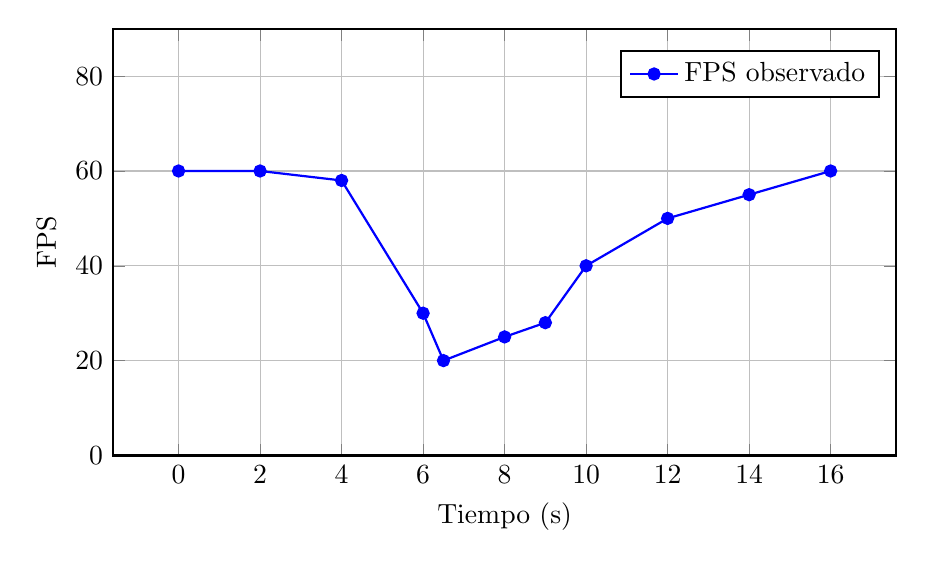
\begin{tikzpicture}
\begin{axis}[
    width=0.95\textwidth,
    height=7cm,
    xlabel={Tiempo (s)},
    ylabel={FPS},
    ymin=0, ymax=90,
    grid=major,
    xtick={0,2,4,6,8,10,12,14,16},
    ytick={0,20,40,60,80},
    legend style={at={(0.98,0.95)},anchor=north east},
    thick
]
\addplot[color=blue, mark=*] coordinates {
    (0,60)   % Inicio estable
    (2,60)
    (4,58)
    (6,30)   % Click logo, caída
    (6.5,20) % Caída máxima
    (8,25)   % Panel informativo
    (9,28)
    (10,40)  % Recuperación progresiva
    (12,50)
    (14,55)
    (16,60)  % Estabilización completa
};
\addlegendentry{FPS observado}
\end{axis}
\end{tikzpicture}
\caption{Evolución del FPS durante la interacción con elementos AR}
\label{fig:fps-evolucion}
\end{figure}


\subsection{Análisis}
Los resultados indican que la experiencia mantiene una tasa de \textbf{50-60 FPS en condiciones normales}, asegurando fluidez inicial (ver Figura \ref{fig:fps-evolucion}). Sin embargo:
\begin{itemize}
    \item \textbf{El mayor impacto ocurre al hacer clic en el logo}, donde se activan múltiples animaciones simultáneas (desaparición del mundo y aparición del modelo principal), reduciendo el FPS hasta 13.
    \item \textbf{El panel informativo genera un impacto menor}, manteniendo los FPS en torno a 25-30, ya que solo añade un plano con texto sin animaciones complejas.
\end{itemize}

